\documentclass{beamer}
\title{Nombre de la Unidad de Aprendizaje}
\date[today]{\today}
\author[Name]{CS1100 - Introducci\'on a Ciencia de la Computaci\'on}
\institute[Department]{UTEC}

\usetheme{lumc}
\usepackage{multicol} % 
%\usepackage{animate}  % animation
\usepackage{amsmath,amsfonts,amssymb} 
\usepackage{listings}
\lstset{basicstyle=\ttfamily,breaklines=true}

\newcommand{\estiloPython}{
\lstset{
    language=Python,
    basicstyle=\fontsize{15}{20}\ttfamily\ttfamily,
    keywordstyle=\color{jpurple}\bfseries,
    stringstyle=\color{red},
    commentstyle=\color{verde},
    morecomment=[s][\color{blue}]{/**}{*/},
    extendedchars=true,
    showspaces=false,
    showstringspaces=false,
    numbers=left,
    numberstyle=\normalsize,
    breaklines=true,
    backgroundcolor=\color{cyan!10},
    breakautoindent=true,
    captionpos=b,
    xleftmargin=0pt,
    tabsize=2
}}

\begin{document}

\begin{frame}
\titlepage
\end{frame}

%%%%%%%%%%%%%%%%%%%%%%%%%%%%%%%%%%%%%%%%%%%%%%%%%%
\section{Motivaci\'on}
%%%%%%%%%%%%%%%%%%%%%%%%%%%%%%%%%%%%%%%%%%%%%%%%%%
\begin{frame}[fragile]{Logro de la Sesi\'on} 
  \begin{block}{Al finalizar esta sesi\'on, estar\'as en la capacidad de:}
    \begin{itemize}[<+- | alert@+>]
      \item desarrollan programas en Python, utilizando funciones y recursividad.
    \end{itemize}
  \end{block}
\end{frame}

%%%%%%%%%%%%%%%%%%%%%%%%%%%%%%%%%%%%%%%%%%%%%%%%%%
\section{Adquisici\'on}
%%%%%%%%%%%%%%%%%%%%%%%%%%%%%%%%%%%%%%%%%%%%%%%%%%
\begin{frame}[fragile]{Dise\~nando funciones:}

{\huge Con los tipos de funciones que hemos estudiado, podemos resolver problemas como:}
\begin{itemize}
\item realizar c\'alculos sucesivos. E.g. calcular la suma de cuadrados de una lista (ver ejemplo 01)
\item validar o verificar. E.g. Encontrar el m\'aximo en una lista (ver ejemplo 02)
\end{itemize}
\end{frame}
%%%%%%%%%%%%%%%%%%%%%%%%%%%%%%%%%%%%%%%%%%%%%%%%%%
\begin{frame}[fragile]{Funci\'on que realiza c\'alculos (ejemplo 01)}

{\Huge Crear una funci\'on para encontrar la suma  de los cuadrados de 1 hasta N.}\\

  \estiloPython
  \begin{lstlisting}[frame = single]
""" codigo que realiza la suma de cuadrados de 1 a N"""
def suma_cuadrados(N):
    suma = 0
    for i in range(1, N + 1):
       suma += i * i
    return suma
N=int(input())
print(suma_cuadrados(N))
  \end{lstlisting}
\end{frame}  

%%%%%%%%%%%%%%%%%%%%%%%%%%%%%%%%%%%%%%%%%%%%%%%%%%
\begin{frame}[fragile]{Funci\'on que realiza validaciones (ejemplo 02)}

{\Huge Encontrar el m\'aximo en una lista}

  \estiloPython
  \begin{lstlisting}[frame = single]
def Max(arr):
    max_ = arr[0]
    for item in arr:
        if item > max_:
            max_ = item
    return max_

i=0
x=int(input("Ingrese un entero (termine con 0): "))
a=list()
while x != 0:
    a.append(x)
    i=i+1
    x=int(input("Ingrese otro numero (termine con 0): "))
print("el numero maximo es: ", Max(a))
  \end{lstlisting}
\end{frame}  

%%%%%%%%%%%%%%%%%%%%%%%%%%%%%%%%%%%%%%%%%%%%%%%%%%

\begin{frame}[fragile]{Algoritmo recursivo}

{\Huge Es un algoritmo que expresa la soluci\'on de un problema en t\'erminos de una llamada a si mismo (llamada recursiva o recurrente}

\begin{figure}
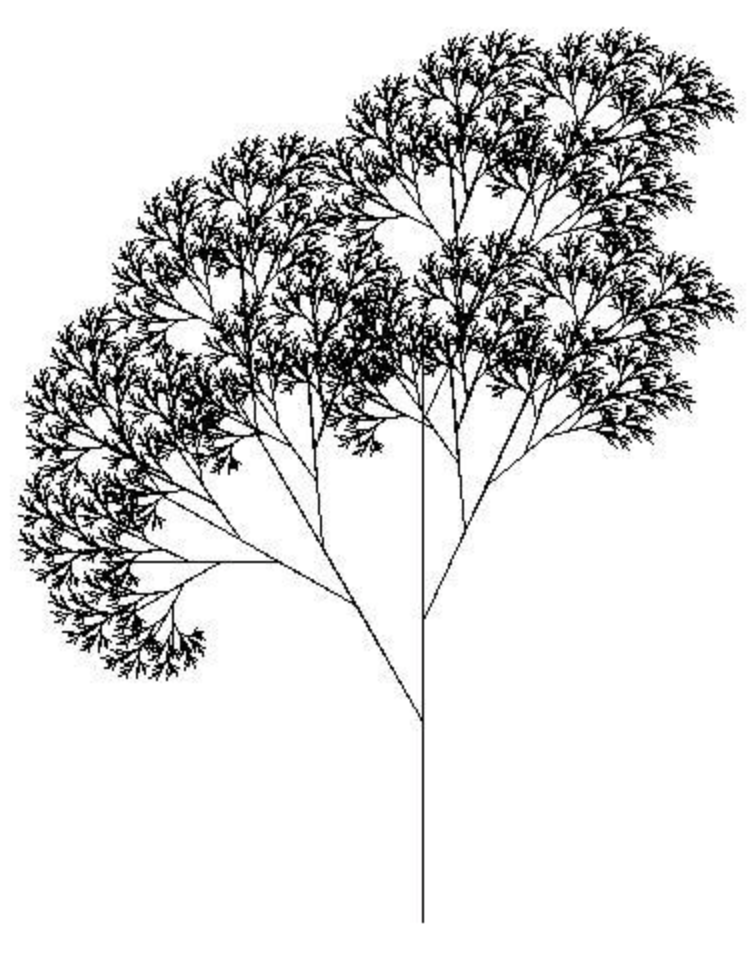
\includegraphics[width=0.4\linewidth]{08.png}
\end{figure}
\end{frame}

%%%%%%%%%%%%%%%%%%%%%%%%%%%%%%%%%%%%%%%%%%%%%%%%%%
\section{Transferencia}
%%%%%%%%%%%%%%%%%%%%%%%%%%%%%%%%%%%%%%%%%%%%%%%%%%
\begin{frame}[fragile]{Autoreferencia}

{\huge La llamada de la funci\'on a si misma hace que se imprima el mensaje un n\'umero indeterminado de veces}

\estiloPython
\begin{lstlisting}[frame = single]
def foo(s):
    print(s)
    foo(s)
foo('hola mundo')
\end{lstlisting}

{\huge El l\'imite de recursividad previene una saturaci\'on de la memoria. Se obtiene el error:\\ RecursionError: maximum recursion depth exceeded while calling a Python object
}
\end{frame}  
  
%%%%%%%%%%%%%%%%%%%%%%%%%%%%%%%%%%%%%%%%%%%%%%%%%%
\begin{frame}[fragile]{Condici\'on de salida:}

{\huge La llamada de la funci\'on a si misma hace que se imprima el mensaje cada vez con un caracter menos}

\estiloPython
\begin{lstlisting}[frame = single]
def foo(s):
    if len(s) == 1:
        print(s)
    else:
        print(s)
        s = s[1:]
        foo(s)
foo('hola mundo')
\end{lstlisting}
\begin{figure}
%\includegraphics[width=0.5\linewidth]{05.png}
\end{figure}
\end{frame}

%%%%%%%%%%%%%%%%%%%%%%%%%%%%%%%%%%%%%%%%%%%%%%%%%%
\begin{frame}[fragile]{Recursividad en algoritmos: Suma de n\'umeros}

{\Large Forma recursiva de calcular la suma de dos n\'umeros naturales a y b.

\begin{equation}
  suma(a,b)=\begin{cases}
    si \ b=0, retornar \ a\\
    Retornar \ 1 + suma(a, b-1)
  \end{cases}
  \end{equation}
  }
  \estiloPython
\begin{lstlisting}[frame = single]
""" suma recursiva"""
def suma(a,b):
    if b == 0:
        return a
    else:
        return 1+suma(a,b-1)

print(suma(21,3))
\end{lstlisting}
\end{frame}

%%%%%%%%%%%%%%%%%%%%%%%%%%%%%%%%%%%%%%%%%%%%%%%%%%
\begin{frame}[fragile]{Recursividad en algoritmos: Suma de cuadrados}

{\huge Forma recursiva de calcular la suma de cuadrados de 1 a N (ver ejemplo 01)}
  \estiloPython
\begin{lstlisting}[frame = single]
def suma_cuadrados(N):
    if(N==1):
        return 1
    else:
        return N*N+suma_cuadrados(N-1)

N=int(input())
print(suma_cuadrados(N))
\end{lstlisting}
\end{frame}

%%%%%%%%%%%%%%%%%%%%%%%%%%%%%%%%%%%%%%%%%%%%%%%%%%

\begin{frame}[fragile]{Recursividad en algoritmos: Factorial de un n\'umero}

{\Large Forma recursiva de calcular el factorial de un n\'umero n.}

{\Large $N! = N \times ( N -1) \times ( N -2 ) \times ... \times 2 \times 1$

\begin{equation}
  factorial(n)=\begin{cases}
    si \ n=1, retornar \ 1\\
    Retornar \ n \times factorial(n-1)
  \end{cases}
\end{equation}
}

\end{frame}

%%%%%%%%%%%%%%%%%%%%%%%%%%%%%%%%%%%%%%%%%%%%%%%%%%
\section{Evaluaci\'on o Cierre}
%%%%%%%%%%%%%%%%%%%%%%%%%%%%%%%%%%%%%%%%%%%%%%%%%%

\begin{frame}[fragile]{Ejercicio 1}
  \begin{block}{Enunciado}
Usando la definici\'on anterior implementar la funci\'on factorial.%def potencia(a, b):\\
  %pass
    \end{block}
%    \estiloPython
%\begin{lstlisting}[frame = single]
%"""esta es la versi\'on iterativa"""
%def factorial\_iterativo(n):
%res = 1
%for i in range(1, n + 1):
%res *= i
%return res
 %        \vspace{.5cm}
  % factorial(n):
 %  if n == 1:
%return 1
%else:
%return $n \times factorial (n-1)$
%\end{lstlisting}

\end{frame} 

%%%%%%%%%%%%%%%%%%%%%%%%%%%%%%%%%%%%%%%%%%%%%%%%%%

\begin{frame}[fragile]{Ejercicio 2}
  \begin{block}{Enunciado}
Crear una funci\'on recursiva que devuelva un numero a elevado a la potencia b.\\
%def potencia(a, b):\\
  %pass
    \end{block}

\end{frame} 

%%%%%%%%%%%%%%%%%%%%%%%%%%%%%%%%%%%%%%%%%%%%%%%%%%
\begin{frame}[fragile]{Ejercicio 3}
  \begin{block}{Enunciado}
 Escribir una funci\'on recursiva que encuentre el mayor elemento de una lista 
%def mayor(l):
    \end{block}

\end{frame} 

%%%%%%%%%%%%%%%%%%%%%%%%%%%%%%%%%%%%%%%%%%%%%%%%%%


\begin{frame}[fragile]{Evaluaci\'on}
  \begin{exampleblock}{Individual Work}
  \begin{itemize}
  \item \href{www.hackerrank.com/cs1100-lab-01
}{www.hackerrank.com/cs1100-lab-01}
  \end{itemize}
\end{exampleblock}    
\end{frame} 

%%%%%%%%%%%%%%%%%%%%%%%%%%%%%%%%%%%%%%%%%%%%%%%%%%

\begin{frame}[fragile]{Cierre} 
  \begin{block}{En esta sesi\'on aprendiste:}
    \begin{itemize}[<+- | alert@+>]
      \item desarrollan programas en Python, utilizando funciones y recursividad.
    \end{itemize}
  \end{block}
\end{frame}


\end{document}